\pdfoptionpdfminorversion=4

\listfiles
\documentclass[notitlepage,preprint,%
amssymb,amsmath,
 aip,jcp%
%groupedaddress,%
%frontmatterverbose,
]{revtex4-1}
%
\usepackage[utf8]{inputenc}
\usepackage[T1]{fontenc}
\usepackage{textcomp}
\usepackage{mathptmx}
\usepackage{bm}%
\usepackage{bbold}
\usepackage{physics}
\usepackage{graphicx}
\usepackage{multirow}
\usepackage{tabularx,booktabs}
\usepackage{color, colortbl}
\usepackage{caption}
\usepackage{subcaption}
\usepackage{subfloat}
\usepackage{xr}
%\externaldocument{../rpapol.tex}
%\definecolor{Gray}{gray}{0.9}
\captionsetup{justification=raggedright}
%
\newcolumntype{Y}{>{\centering\arraybackslash}X}
%\nofiles
\expandafter\ifx\csname package@font\endcsname\relax\else
 \expandafter\expandafter
 \expandafter\usepackage
 \expandafter\expandafter
 \expandafter{\csname package@font\endcsname}%
\fi
\hyphenation{title}
%
\begin{document}
\title{Human PNP free energies}
\author{}
%
\date{\today}
\maketitle

%\tableofcontents

\section{Computational details of the free energy calculations}
The free energy calculations were performed within the Transition path sampling 
(TPS) method \cite{Balasubramani22JPhysChemB126p5413} for the reaction catalyzed 
by the human PNP enzyme. The order parameter ($\xi$) for both the constrained
and unconstrained PNP systems was chosen to be d$_{\text{NC}}-$d$_{\text{OC}}$.   
A reactive trajectory from the TPS ensemble was selected for both the constrained 
and unconstrained PNP systems as the starting point for the equilibrium sampling 
of configurations corresponding to order parameter values within the range of 
$\left[-3.0,3.0\right]$ {\AA}. This order parameter range was divided into 30 
overlapping windows with an overlap of 0.08 {\AA} between neighboring windows. 
Within each window $i$ (defined by the set of order parameter values 
$\left[\xi^{min}_i,\xi^{max}_i\right]$) configurations are sampled starting 
from a time frame in the TPS reactive trajectory with an order parameter $\bar{\xi}$
that satisfies $\xi^{min}_i\le \bar{\xi} \le \xi^{max}_{i}$. Using the shooting 
algorithm \cite{Bolhuis02AnnRevPhysChem53p291,dellago02AdvChemPhys123} the momenta 
of all the atoms of the enzymatic system are perturbed and dynamics is propagated 
to obtain a short 20 fs trajectory (10 fs forwards and backwards from the 
shooting point) with a time step of 1 fs. After sampling 3000 trajectories 
within each window, the converged probability distribution
of the order parameter ($w_i$) is obtained as normalized histograms. 
The free energy ($F_i = -k_BT\log(w_i) + c_i$) calculated within each window 
is shifted to obtain a continuous free energy profile.

\begin{figure}[ht!]
  \centering
  \begin{minipage}[b]{0.48\linewidth}
    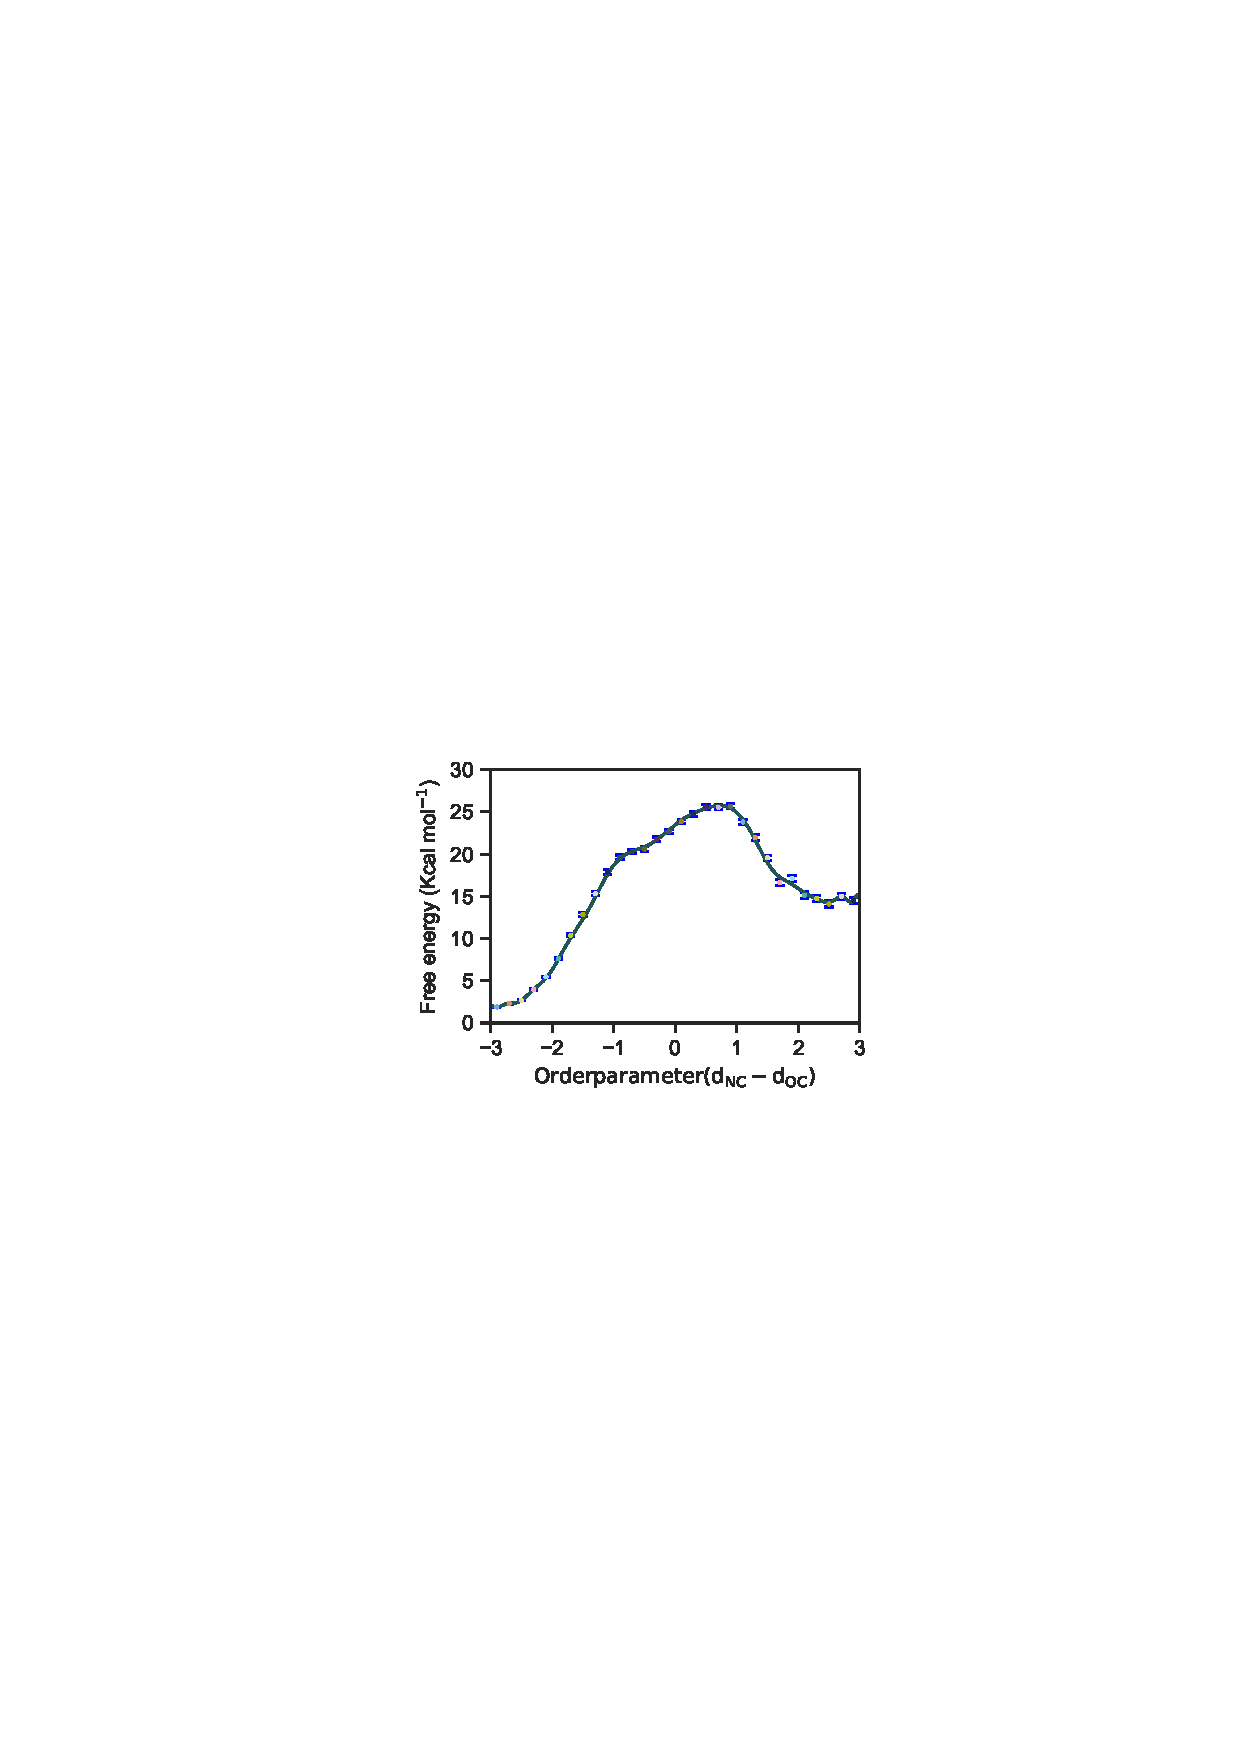
\includegraphics[scale=1.0]{figures/pnp-uncons-fenergy.png}
    %\caption{Distribution of the order parameter}
    %\label{fig:dist}
  \end{minipage}
  \quad
  \begin{minipage}[b]{0.48\linewidth}
    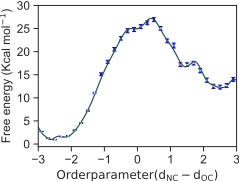
\includegraphics[scale=1.0]{figures/pnp-cons-fenergy.png}
    %\caption{Free energy using Boltzmann inversion}
    %\label{fig:fenergy}
  \end{minipage}
  \caption{Free energy profile for the unconstrained (left) and constrained (right) PNP systems 
  calculated using the TPS based method. Standard deviations are calculated using the bootstrapping 
method and denoted as blue error bars while the continuous black curve represents the polynomial 
fitting function.}
\label{fig:fenergy}
\end{figure}

From Fig. \ref{fig:fenergy} the free energy barriers for the unconstrained and constrained PNP systems 
are calculated to be $23$ kcal mol$^{-1}$ and 26 kcal mol$^{-1}$, respectively. 
>>>>>>> cf17cce75ea22f9894e5fc14e500e3b80aba045c

%\bibliographystyle{unsrt}
\bibliography{pnp-free-energy}
\end{document}
